\documentclass[12pt]{report}
\usepackage[utf8]{inputenc}
\usepackage[russian]{babel}
%\usepackage[14pt]{extsizes}
\usepackage{listings}
\usepackage{graphicx}
\usepackage{amsmath,amsfonts,amssymb,amsthm,mathtools} 
\usepackage{float}

% Для листинга кода:
\lstset{ %
language=C++,                 % выбор языка для подсветки (здесь это С)
basicstyle=\small\sffamily, % размер и начертание шрифта для подсветки кода
numbers=left,               % где поставить нумерацию строк (слева\справа)
numberstyle=\tiny,           % размер шрифта для номеров строк
stepnumber=1,                   % размер шага между двумя номерами строк
numbersep=5pt,                % как далеко отстоят номера строк от подсвечиваемого кода
showspaces=false,            % показывать или нет пробелы специальными отступами
showstringspaces=false,      % показывать или нет пробелы в строках
showtabs=false,             % показывать или нет табуляцию в строках
frame=single,              % рисовать рамку вокруг кода
tabsize=2,                 % размер табуляции по умолчанию равен 2 пробелам
captionpos=t,              % позиция заголовка вверху [t] или внизу [b] 
breaklines=true,           % автоматически переносить строки (да\нет)
breakatwhitespace=false, % переносить строки только если есть пробел
escapeinside={\#*}{*)}   % если нужно добавить комментарии в коде
}

% Для измененных титулов глав:
\usepackage{titlesec, blindtext, color} % подключаем нужные пакеты
\definecolor{gray75}{gray}{0.75} % определяем цвет
\newcommand{\hsp}{\hspace{20pt}} % длина линии в 20pt
% titleformat определяет стиль
\titleformat{\chapter}[hang]{\Huge\bfseries}{\thechapter\hsp\textcolor{gray75}{|}\hsp}{0pt}{\Huge\bfseries}


% plot
\usepackage{pgfplots}
\usepackage{filecontents}
\usetikzlibrary{datavisualization}
\usetikzlibrary{datavisualization.formats.functions}
\begin{filecontents}{LevR.dat}
100 45504
200 344852
300 1626090
400 4410053
500 8809530
600 15523926
700 27314819
800 36896674
900 151438792
1000 253111941
\end{filecontents}

\begin{filecontents}{LevT.dat}
100 50613
200 254889
300 1164803
400 3277843
500 6466829
600 10441740
700 20235150
800 27982176
900 115139281
1000 199701561
\end{filecontents}

\begin{filecontents}{DamLevR.dat}
100 22663
200 189215
300 937882
400 2605948
500 5077237
600 9041331
700 15047492
800 20829956
900 85256627
1000 158414218
\end{filecontents}



\begin{filecontents}{LevR1.dat}
101 45393
201 386372
301 1557256
401 4538718
501 9009942
601 15214595
701 26603522
801 37648086
901 139235577
1001 278285719
\end{filecontents}

\begin{filecontents}{LevT1.dat}
101 35265
201 364594
301 1113414
401 3314034
501 6511456
601 11947585
701 20274021
801 26844301
901 136919210
1001 212082553
\end{filecontents}

\begin{filecontents}{DamLevR1.dat}
101 38152
201 196174
301 919775
401 2652528
501 5171817
601 10328122
701 15001586
801 20867237
901 108043316
1001 165932409
\end{filecontents}



\begin{document}
%\def\chaptername{} % убирает "Глава"
\begin{titlepage}
	\centering
	{\scshape\LARGE МГТУ им. Баумана \par}
	\vspace{3cm}
	{\scshape\Large Лабораторная работа №4\par}
	\vspace{0.5cm}	
	{\scshape\Large По курсу: "Анализ алгоритмов"\par}
	\vspace{1.5cm}
	{\huge\bfseriesПараллельное умножение матриц\par}
	\vspace{2cm}
	\Large Работу выполнила: Лаврова Анастасия, ИУ7-55Б\par
	\vspace{0.5cm}
	\LargeПреподаватели:  Волкова Л.Л., Строганов Ю.В.\par

	\vfill
	\large \textit {Москва, 2019} \par
\end{titlepage}

\tableofcontents

\newpage
\chapter*{Введение}
\addcontentsline{toc}{chapter}{Введение}
Цель работы: изучение алгоритмов умножения матриц. В данной лабораторной работе рассматривается стандартный алгоритм умножения матриц, алгоритм Винограда и модифицированный алгоритм Винограда.  Также требуется изучить рассчет сложности алгоритмов, получить навыки в улучшении алгоритмов.
Эти алгоритмы активно применяются во всех областях, применяющих линейную алгебру, таких как:
\begin{itemize}
	\item компьютерная графика
	\item физика
	\item экономика
\end{itemize}


В ходе лабораторной работы предстоит:
\begin{itemize}
	\item  Изучение и реализация параллельного алгоритма Винограда для умножения матриц 
	\item Сравнить зависимость времени работы алгоритма от числа параллельных потоков исполнения и размера матриц 
	\item Провести сравнение стандартного и параллельного алгоритма.
\end{itemize}





\chapter{Аналитическая часть}
Матрица - математический объект, эквивалентный двумерному массиву. Числа располагаются в матрице по строкам и столбцам. Если число столбцов в первой матрице совпадает с числом строк во второй, то эти две матрицы можно перемножить. У произведения будет столько же строк, сколько в первой матрице, и столько же столбцов, сколько во второй.


\section{Алгоритм Винограда}
Рассмотрим два вектора $V = (v1, v2, v3, v4)$ и $W = (w1, w2, w3, w4)$. Их скалярное произведение равно: 

$ V \cdot W=v_1 \cdot w_1 + v_2 \cdot w_2 + v_3 \cdot w_3 + v_4 \cdot w_4$ \\

Это равенство можно переписать в виде: \\
$V \cdot W=(v_1 + w_2) \cdot (v_2 + w_1) + (v_3 + w_4) \cdot (v_4 + w_3) - v_1 \cdot v_2 - v_3 \cdot v_4 - w_1 \cdot w_2 - w_3 \cdot w_4$\\

Менее очевидно, что выражение в правой части последнего равенства допускает предварительную обработку: его части можно вычислить заранее и запомнить для каждой строки первой матрицы и для каждого столбца второй. 
Это означает, что над предварительно обработанными элементами нам придется выполнять лишь первые два умножения и последующие пять сложений, а также дополнительно два сложения. 

\section{Параллельный алгоритм Винограда }
Трудоемкость алгоритма Винограда имеет сложность $O(nmk)$ для умножения матриц $n1 \times m1$ на $n2 \times m2$. Чтобы улучшить алгоритм, следует распараллелить ту часть алгоритма, которая содержит 3 вложенных цикла.\\

	Вычисление результата для каждой строки не зависит от результата выполнения умножения для других строк. Поэтому можно распараллелить часть кода, где происходят эти действия. Каждый поток будет выполнять вычисления определенных строк результирующей матрицы.
	
\section{Распараллеливание задачи}
В рамках данной лабораторной работы производилось распараллеливание задачи по потокам. В CPU для данной цели используются treads.  \\
	
	CPU – central processing unit – это универсальный процессор, также именуемый процессором общего назначения. Он оптимизирован для достижения высокой производительности единственного потока команд. Доступ к памяти с данными и инструкциями происходит преимущественно случайным образом.
Для того, чтобы повысить производительность CPU еще больше, они проектируются специально таким образом, чтобы выполнять как можно больше инструкций параллельно. Например для этого в ядрах процессора используется блок внеочередного выполнения команд.	
Но несмотря на это, CPU все равно не в состоянии осуществить параллельное выполнение большого числа инструкций, так как расходы на распараллеливание инструкций внутри ядра оказываются очень существенными. Именно поэтому процессоры общего назначения имеют не очень большое количество исполнительных блоков.


\subsection{Вывод}
Были рассмотрены поверхностно стандартная и параллельная реализации алгоритма Винограда.


\chapter{Конструкторская часть}
\textbf{Требования к вводу:}\\
На вход подаются две матрицы и их размерности\\
\textbf{Требования к программе:}\\
Корректное умножение двух матриц \\

На рис. \ref{fig:def} представлена IDEF0 диаграмма умножения двух матриц:
	
	\begin{figure}[h]
        	\begin{center}
        		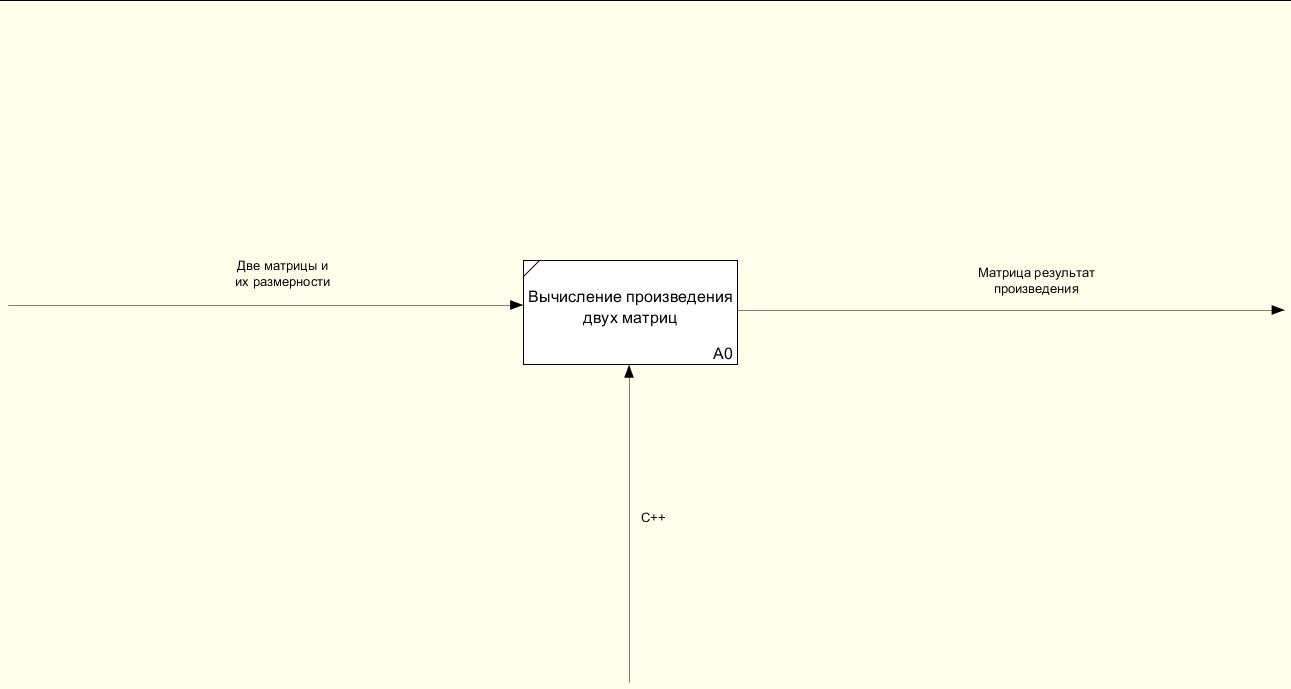
\includegraphics[scale=0.6]{idef}
        		\caption{IDEF0 диаграмма умножения двух матриц}
        		\label{fig:def}
        	\end{center}
        \end{figure}


\section{Схемы алгоритмов}

На рис. \ref{fig:def} представлена  схема стандартного алгоритма Винограда:
	\begin{figure}[h]
        	\begin{center}
        		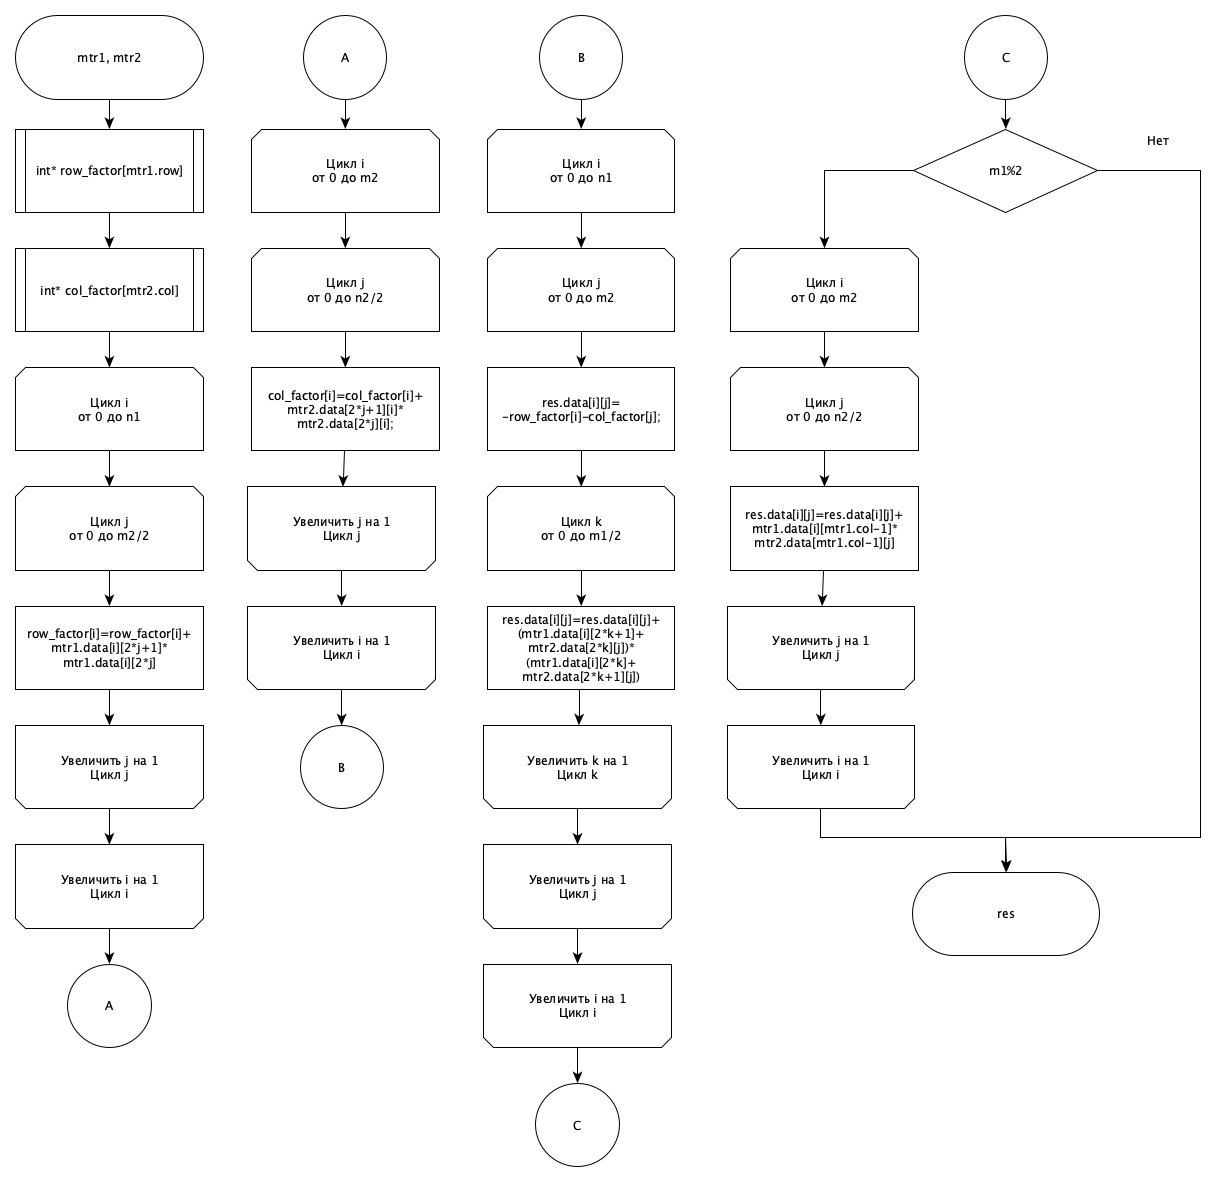
\includegraphics[scale=0.32]{standart_vinograd2}
        		\caption{Cхема стандартного алгоритма Винограда}
        		\label{fig:def}
        	\end{center}
        \end{figure}
        
На рис. \ref{fig:def} представлена схема распараллеленого алгоритма Винограда:
	\begin{figure}[h]
        	\begin{center}
        		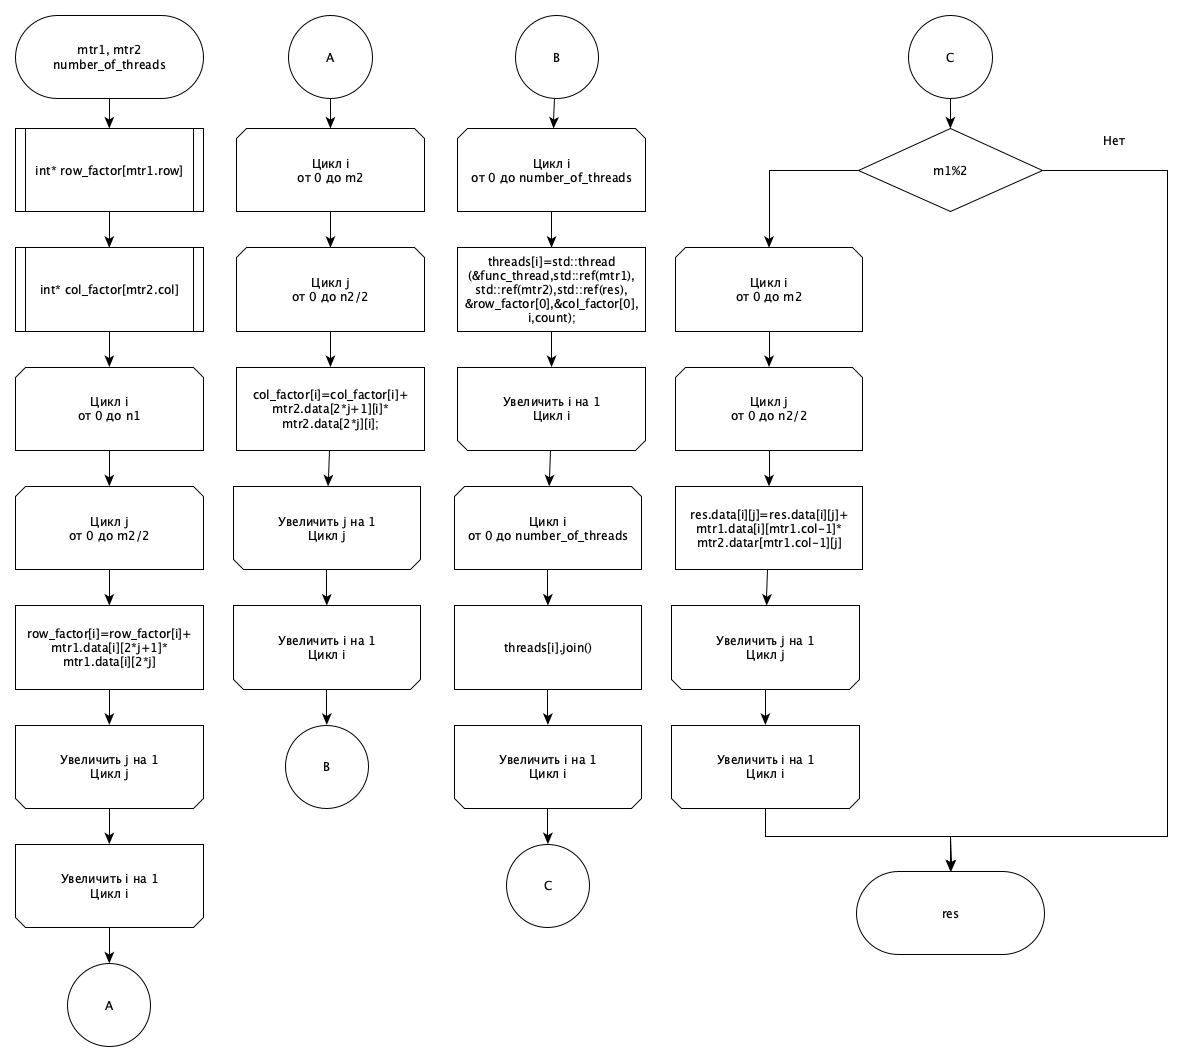
\includegraphics[scale=0.32]{parallel_vinograd2}
        		\caption{Схема распараллеленого алгоритма Винограда}
        		\label{fig:def}
        	\end{center}
        \end{figure}
        
На рис. \ref{fig:def} ппредставлена схема фнкции параллельного вычисления матрицы:
	\begin{figure}[h]
        	\begin{center}
        		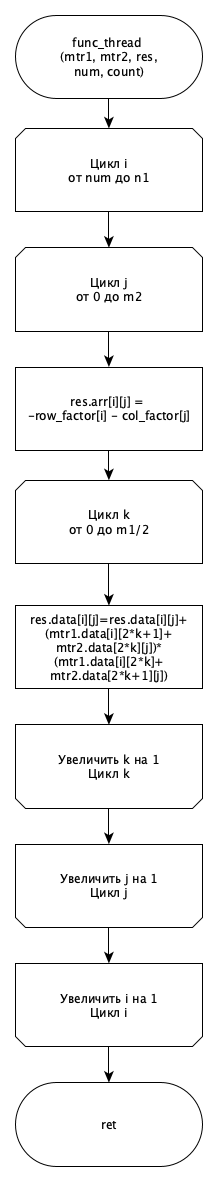
\includegraphics[scale=0.32]{parallel_func}
        		\caption{Схема распараллеленого алгоритма Винограда}
        		\label{fig:def}
        	\end{center}
        \end{figure}

\chapter{Технологическая часть}
\section{Выбор ЯП}
Для реализации программ я выбрала язык программирования C++, так имею большой опыт работы с ним. Среда разработки - Visual Studio. \\

Для отключения оптимизации компилятора указан флаг «-o0».\\
Для работы с потоками используется библиотека поддержки потоков std::thread. \\
Наблюдатель joinable  проверяет потенциальную возможность работы потока в параллельном контексте.\\
Операция join ожидает завершения потока. \\

Для замера процессорного времени используется функция, возвращающая количество тиков.\\

\begin{lstlisting}[label=some-code,caption=Функция получения тиков]
unsigned long long getTicks(void)
{
    unsigned long long d;
    __asm__ __volatile__ ("rdtsc" : "=A" (d) );
    return d;
}

\end{lstlisting}

\section{Реализация алгоритма}

\begin{lstlisting}[label=s,caption=Стандартный алгоритм Винограда]
Matrix Matrix::vinograd_mult(const Matrix &mtr1, const Matrix &mtr2)
{
    Matrix res(mtr1.row, mtr2.column);

    int row_factor[mtr1.row];
    int col_factor[mtr2.column];

    for(int i = 0; i < mtr1.row; i++)
    {
        row_factor[i] = 0;
        for(int j = 0; j < mtr1.column / 2; j++)
        {
            row_factor[i] = row_factor[i] + mtr1.data[i][2 * j] * mtr1.data[i][2 * j + 1];
        }
    }

    for(int i = 0; i < mtr2.column; i++)
    {
        col_factor[i] = 0;
        for(int j = 0; j < mtr2.row / 2; j++)
        {
            col_factor[i] = col_factor[i] + mtr2.data[2 * j][i] * mtr2.data[2 * j + 1][i];
        }
    }

    for(int i = 0; i < mtr1.row; i++)
    {
        for(int j = 0; j < mtr2.column; j++)
        {
            res.data[i][j] = -row_factor[i] - col_factor[j];
            for(int k = 0; k < mtr1.column / 2; k++)
            {
                res.data[i][j] = res.data[i][j] +
                                    (mtr1.data[i][2 * k + 1] + mtr2.data[2 * k][j]) *
                                    (mtr1.data[i][2 * k] + mtr2.data[2 * k + 1][j]);
            }
        }
    }
    
    if(mtr1.column % 2)
    {
        for(int i = 0; i < mtr1.row; i++)
            for(int j = 0; j < mtr2.column; j++)
                res.data[i][j] = res.data[i][j] + mtr1.data[i][mtr1.column - 1] * mtr2.data[mtr1.column - 1][j];
    }

    return res;
}
\end{lstlisting}


В листинге \ref{p} представлен параллельный алгоритм Винограда:\\
	
	Можно заметить, что вычисление результата для каждой строки происходит независимо от результата выполнения умножения для других строк. Поэтому возможно распараллелить участок кода, соответстующий строкам 24-32 листинга \ref{s}. Каждый поток будет выполнять вычисление некоторых строк результирующей матрицы. Это сделано потому, что проход по строкам матрицы является более эффективным с точки зрения организации данных в памяти.

	\begin{lstlisting}[label=p,caption=Параллельный алгоритм Винограда]
Matrix Matrix::vinograd_mult_multithreading(const Matrix &mtr1, const Matrix &mtr2, int count)
{

    Matrix res(mtr1.row, mtr1.column);

    int row_factor[mtr1.row];
    int col_factor[mtr1.column];

    for(int i = 0; i < mtr1.row; i++)
    {
        row_factor[i] = 0;
        for(int j = 0; j < mtr1.column / 2; j++)
        {
            row_factor[i] = row_factor[i] + mtr1.data[i][2 * j + 1] * mtr1.data[i][2 * j];
        }
    }

    for(int i = 0; i < mtr1.column; i++)
    {
        col_factor[i] = 0;
        for(int j = 0; j < mtr1.column / 2; j++)
        {
            col_factor[i] = col_factor[i] + mtr1.data[2 * j + 1][i] * mtr1.data[2 * j][i];
        }
    }

    std::thread threads[count];

    for(int i = 0; i < count; i++)
    {
        threads[i] = std::thread(&func_thread, std::ref(mtr1), std::ref(mtr1), std::ref(res), &row_factor[0], &col_factor[0], i, count);
    }
    
    for(int i = 0; i < count; i++)
    {
        if(threads[i].joinable())
        {
            threads[i].join();
        }
    }

    if(mtr1.column % 2)
    {
        for(int i = 0; i < mtr1.row; i++)
            for(int j = 0; j < mtr1.column; j++)
                res.data[i][j] = res.data[i][j] + mtr1.data[i][mtr1.column - 1] * mtr1.data[mtr1.column - 1][j];
    }

    return res;
}
\end{lstlisting}

В листинге \ref{pf} представлено распараллеленное вычисление тройного цикла:

	\begin{lstlisting}[label=pf,caption=Распараллеленный тройной цикл]
void func_thread(const Matrix &mtr1, const Matrix &mtr2, Matrix &res,  int* row_factor,  int* col_factor, int num, int count)
{
    for(int i = num; i < mtr1.row; i += count)
    {
        for(int j = 0; j < mtr2.column; j++)
        {
            res.data[i][j] = -row_factor[i] - col_factor[j];
            for(int k = 0; k < mtr1.column / 2; k++)
            {
                res.data[i][j] = res.data[i][j] + (mtr1.data[i][2 * k + 1] + mtr2.data[2 * k][j]) * mtr1.data[i][2 * k] + mtr2.data[2 * k + 1][j];
            }
        }
    }
}
\end{lstlisting}



\chapter{Исследовательская часть}

\section{Постановка эксперимента}

Были проведены исследования зависимости времени работы трех алгоритмов от размеров перемножаемых матриц и количества использованных потоков. Замеры времени проводились для матриц четной размерности размером от 100 до 1000 с шагом 100 и матриц нечетной размерности размером от 101 до 1001 с шагом 100. Количество потоков - от 1 до 32, т.к. компьютер, на котором проводились вычисления, содержит 8 логических ядра.\\
	
	 Временные замеры проводятся путём многократного проведения эксперимента и деления результирующего времени на количество итераций эксперимента. \\

\section{Сравнительный анализ на основе замеров времени работы алгоритмов}

На рис. \ref{chet} представлен график времени работы алгоритма на матрицах четной размерности:
	
	\begin{figure}[h]
        	\begin{center}
        		{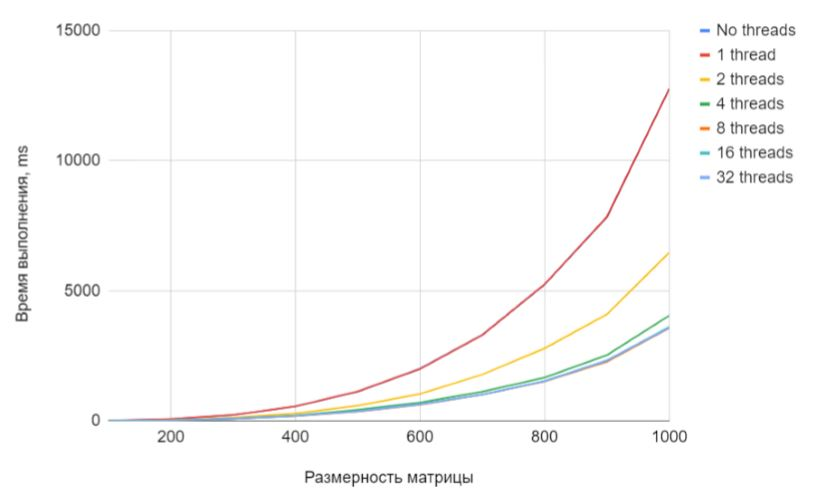
\includegraphics[scale = 0.8]{diag_chet2}}
        		\caption{График времени работы на матрицах четной размерности}
        		\label{chet}
        	\end{center}
        \end{figure}

	\newpage
	На рис. \ref{nechet} представлен график времени работы алгоритма на матрицах нечетной размерности:
	
	\begin{figure}[H]
        	\begin{center}
        		{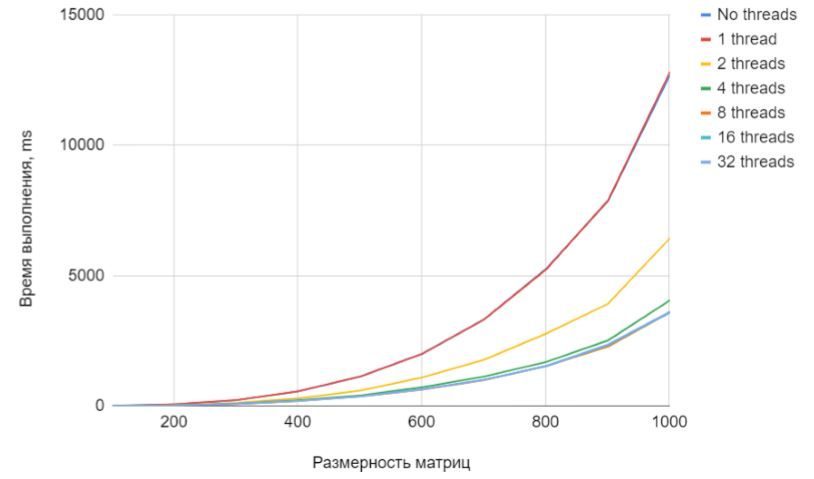
\includegraphics[scale = 0.8]{diag_nechet2}}
        		\caption{График времени работы на матрицах нечетной размерности}
        		\label{nechet}
        	\end{center}
        \end{figure}
        
 

\section{Вывод}

Эксперименты замера времени показали, что при последовательной и параллельной (с одним рабочим потоком) реализациях оптимизированного алгоритма Винограда совсем немного выигрывает последовательная реализация (в ней не тратится время на выделение рабочего потока).
       
        При сравнении замеров времени для параллельной реализации алгоритма с 1, 2, 4, 8, 16 и 32 рабочими потоками выяснилось, что максимальная производительность достигается на 8-ми рабочих потоках , что равно количеству логических потоков компьютера, на котором производились замеры. Выполнение алгоритма на 8-ми рабочих потоках быстрее в 3,82 раз, по сравнению с выполнением на 1-м потоке для матриц размера $1000 \times 1000$. При большем количестве рабочих потоков происходит небольшое падение производительности (тратится время на создание новых рабочих потоков, но вычисления будут производиться с той же скоростью, что и при 8 рабочих потоках).





\chapter*{Заключение}
\addcontentsline{toc}{chapter}{Заключение}
В ходе работы был изучен параллельный алгоритм умножения матриц: алгоритм Винограда. Выполнено сравнение зависимости всех рассматриваемых алгоритмов от числа параллельных потоков и размера матриц. В ходе исследования было установлено, что многопоточный алгоритм Винограда выполняется быстрее, чем стандартный алгоритм.




\end{document}